\section{Summary of Metrics}\label{analysis}

\cite{lanza2002beyond} zuerst gibts auch metriken die entweder class metirken oder methoden metirken oder attribute metriken sind. kann man so klassifzieren

- wie grenze ich mich ab von denen von related work

- evaluation possibilities

- The chapter in which the metrics are enumerated in general and then (maybe) two are picked out and discussed in detail

- introduction to some metrics, properties, studies that deal with fault-proneness and investigate the issue of FP

- Some of these metrics are based simply on counting the number of interactions

- add path connectivity class cohesion (PCCC) to table

- metrics table:

\begin{table}
	\caption{Metrics.}~\label{tab:metrics}
	
	\setlength\tabcolsep{3pt}
	\renewcommand{\arraystretch}{1.4}% for the vertical padding
	\begin{tabularx}{\columnwidth}{ | c | p{5.8cm} || c | }
		\hline
		Abbrevation & Definition & Sources \\ \hline\hline
		CBO & Coupling between Objects for a class is .. Coupling between Objects for a class is ..Coupling between Objects for a class is ..Coupling between Objects for a class is ..Coupling between Objects for a class is ..& \cite{b14chidamber1994metrics} \\ \hline
		LOC & Lack of Cohesion counts ..  & \cite{b15chidamber1991towards} \\ \hline
		DOI & Depth of Inheritance .. & \cite{b15chidamber1991towards} \\ \hline
		... & ... & ... \\ \hline
	\end{tabularx}
\end{table}


\subsection{A Precise Method-Method Interaction-Based Cohesion Metric for Object-Oriented Classes}

\textbf{1st method} Fault Prediction and the Discriminative Powers of Connectivity-Based
Object-Oriented Class Cohesion Metrics \cite{b8al2012precise} ::: 
- explain as an example the Precise Method-Method Interaction-Based Cohesion Metric for Object-Oriented Classes from paper \cite{b8al2012precise}.

- explain method: the proposed class cohesion metric is based on counting the number of possible paths in graph that represents the connectivity pattern of the class members

- relevance of methods, attributes in classes and their connectivity, figure \ref{fig1}, figure \ref{fig2}, figure \ref{fig3}.

- search for other graphical representation ($\rightarrow$ java code snippet)

- benefits and limitations of the method (maybe to results?)


\begin{figure}[htbp]
	\centerline{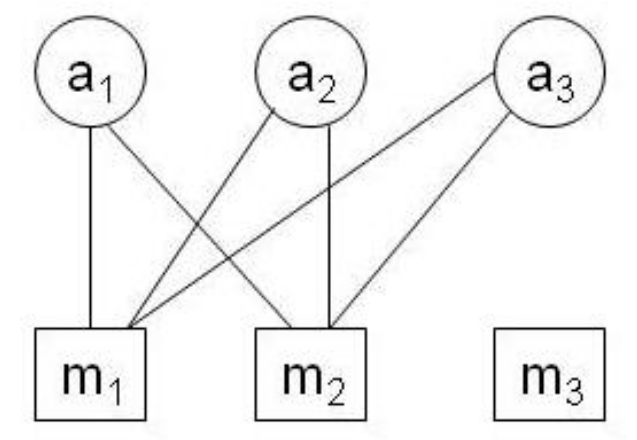
\includegraphics[width=0.2\textwidth]{pictures/am.png}}
	\caption{Sample representative graph for a hypothetical class \cite{b3al2012fault}.}
	\label{fig1}
\end{figure}

\begin{figure}[htbp]
	\centerline{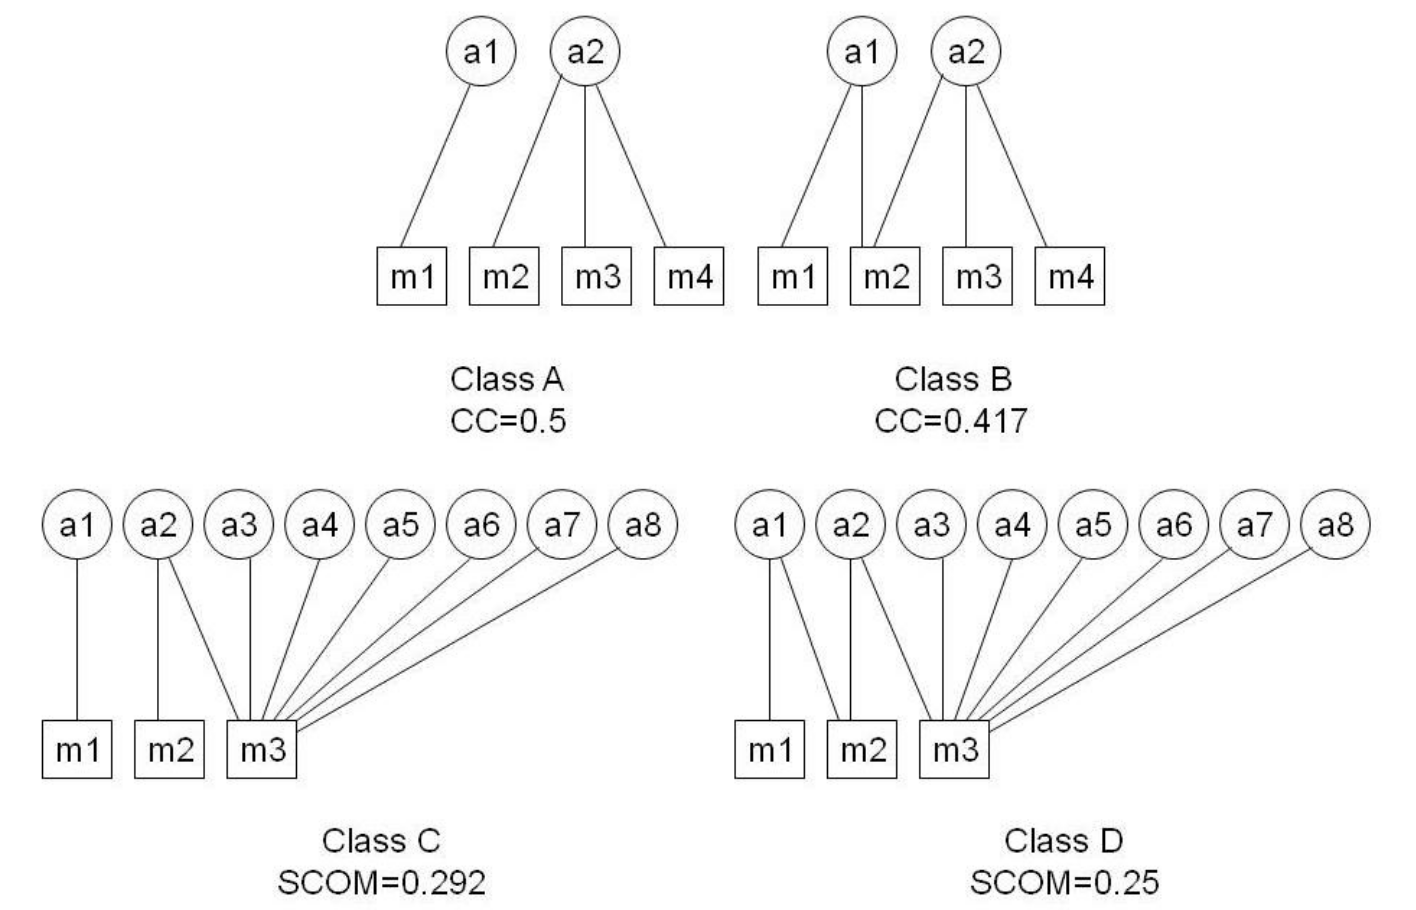
\includegraphics[width=0.4\textwidth]{pictures/am2.png}}
	\caption{Classes with different method-method connectivity patterns \cite{b3al2012fault}.}
	\label{fig2}
\end{figure}

\begin{figure}[htbp]
	\centerline{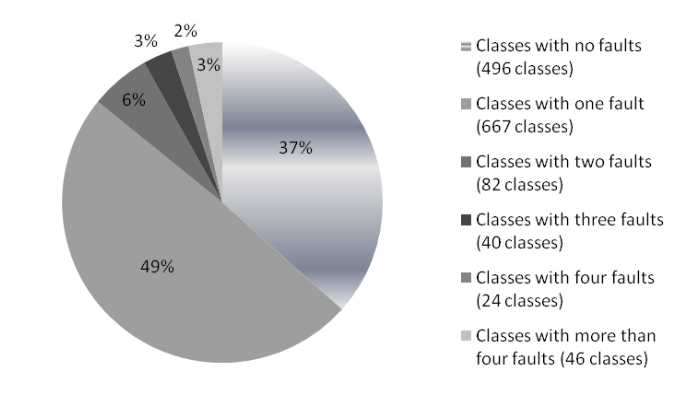
\includegraphics[width=0.5\textwidth]{pictures/circle.png}}
	\caption{Sample representative graph for a hypothetical class \cite{b3al2012fault}.}
	\label{fig3}
\end{figure}


\subsection{A Bayesian network}

- is a concise representation of a joint probability distribution on a set of statistical variables

- encoded as an acyclic graph of nodes and directed edges \cite{b9pai2007empirical}. 

- how Bayesian methods can be used for assessing software fault content and fault proneness

- dependent variables, which serve as surrogate metrics of software quality: fault content and fault proneness.

- a BN model whose underlying representation is the generalized linear model (infos to the model)

- (maybe) definition probabilistic network (acyclic graph $G=(V,E)$; A set $S$, of (prior) conditional probability distributions)

- (maybe) given a BN structure, the joint probability distribution over $X$ is encoded as

\begin{math}
	p(X)= \prod_{i=1}^{n}p(X_i|P_{ax_i})
\end{math}

- some maths: short summary of the mathematical aspects!?

- explain the variables and the fault-pron context

\begin{figure}[htbp]
	\centerline{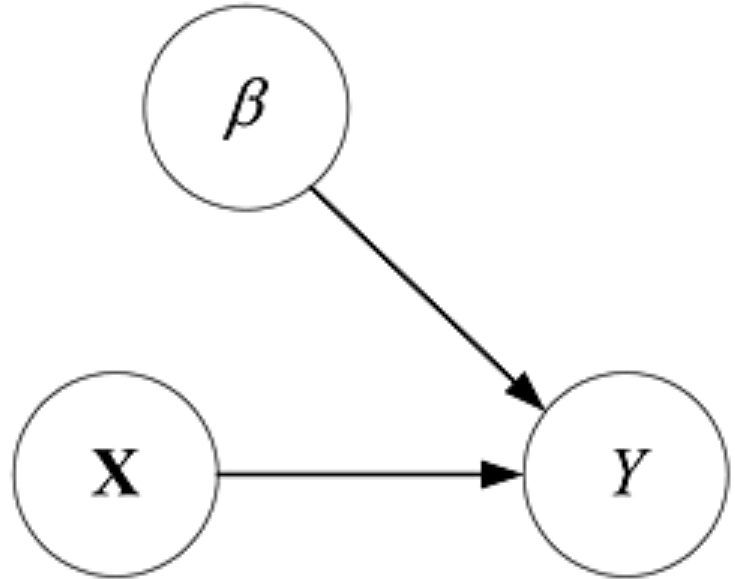
\includegraphics[width=0.2\textwidth]{pictures/bn1.png}}
	\caption{BN representation of a general linear model.}
	\label{fig1bn}
\end{figure}

- model parameters from \cite{b9pai2007empirical}: (somehow merge with table!?; until now almost copied out from paper)

\begin{itemize}
	\item[1.] Weighted methods per class (WMC): The number of methods implemented in a given class.
	\item[2.] Depth of inheritance tree (see table)
	\item[3.] Response for class (RFC): Number of methods implemented within a class plus the number of methods accessible to an object class due to inheritance. (Traditionally, it represents the number of methods that an object of a given class can execute in response to a received message \cite{b9pai2007empirical}.)
	\item[4.] Number of children (NOC): The number of classes that directly inherit from a given class.
	\item[6.] Coupling between object classes (CBO): The number of distinct non-inheritance related classes to which a given class is coupled. (i.e., when a given class uses the methods or attributes of the coupled class \cite{b9pai2007empirical}.)
	\item[7.] Lack of cohesion in methods (LCOM): A measure of the degree to which a class represents single or multiple abstractions. There are varying definitions for LCOM. (i.e., by computing the average percentage of methods in a given class using each attribute of that class, and then subtracting that percentage from 100 percent \cite{b9pai2007empirical}.)
	\item[8.] Source lines of code (SLOC): This is measured as the total lines of source code in the class and serves as a measure of class size.
\end{itemize}

- dependencies between metrics and impact

\begin{figure}[htbp]
	\centerline{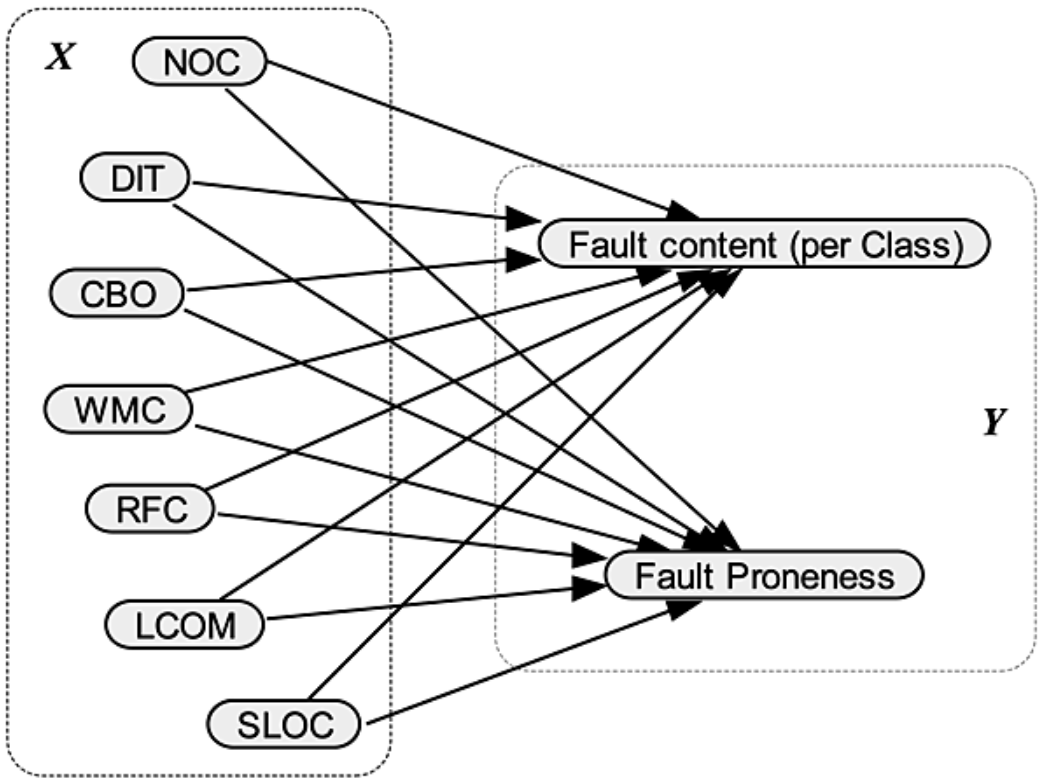
\includegraphics[width=0.4\textwidth]{pictures/bn2.png}}
	\caption{BN model for defect content and defect proneness analysis.}
	\label{fig2bn}
\end{figure}

- summary of study/paper; note important aspects

- RESULTS 

- BN: the results of performing multiple regression, the metrics WMC, CBO, RFC, and SLOC are very significant for assessing both fault content and fault proneness

- this specific set of predictors is very significant for assessing fault content and fault proneness in large software systems

- it was observed that import coupling (that count the number of other classes called by a class) metrics are strongly associated with fault
pron and predict faulty classes with high accuracy

- Associate refactoring to the last sections
